\clearpage

\subsection{Preselection Yields}
\label{sec:yields}

The  dilepton mass spectra for the $ee$ and $\mu\mu$ final states are shown in 
Figure~\ref{fig:dilmass}, after applying the preselection of Sec.~\ref{sec:eventSelection}, except for the dilepton mass requirement.
For all MC plots and tables, the yields are normalized to \lumi\ using the cross-sections
from Reference~\cite{ref:xsec}.
%assuming 100\% 
%using trigger efficiency as described in section \ref{sec:trigSel}.
%Add statement about overflow
For these plots and all others in this note, the last bin contains the overflow.


\begin{figure}[hbt]
  \begin{center}
	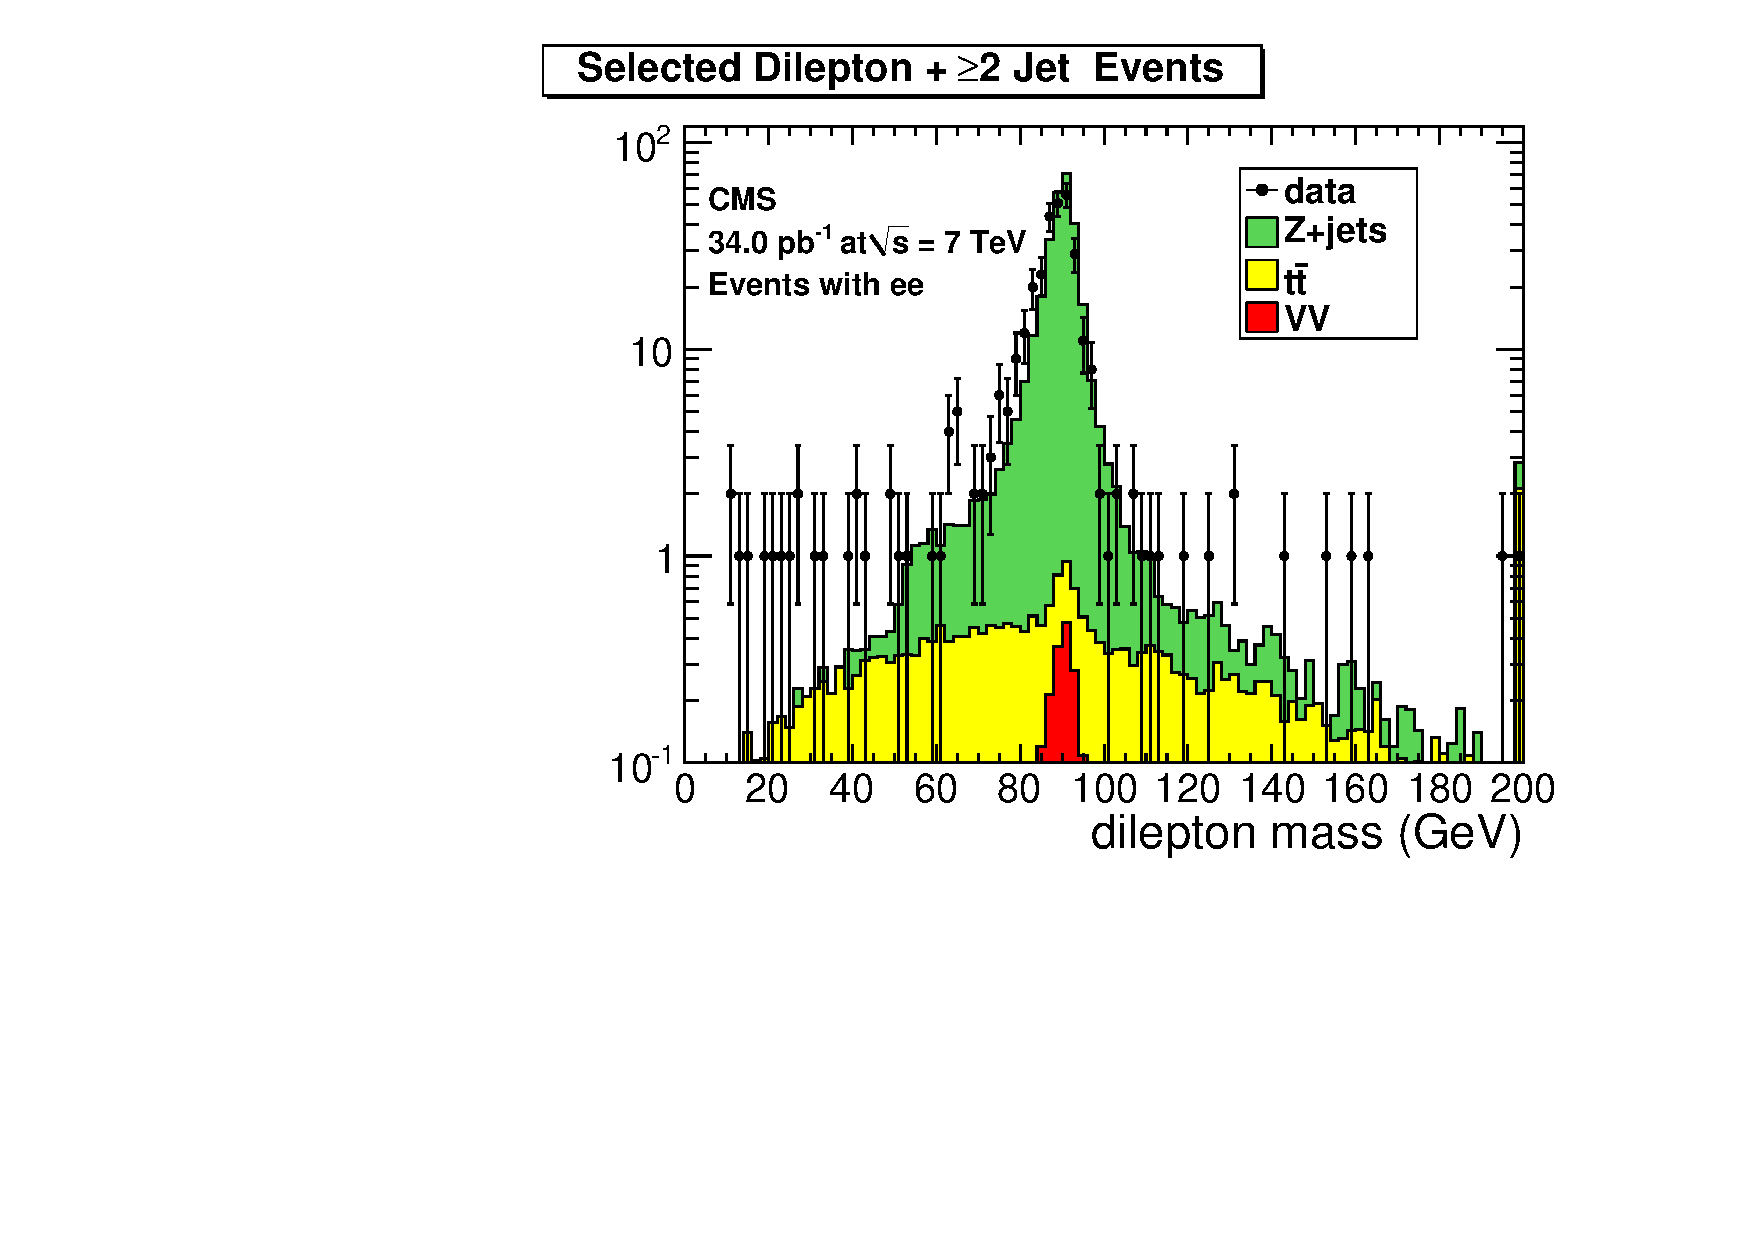
\includegraphics[width=0.48\linewidth]{plots/hdilmass_ee_allj.pdf}
	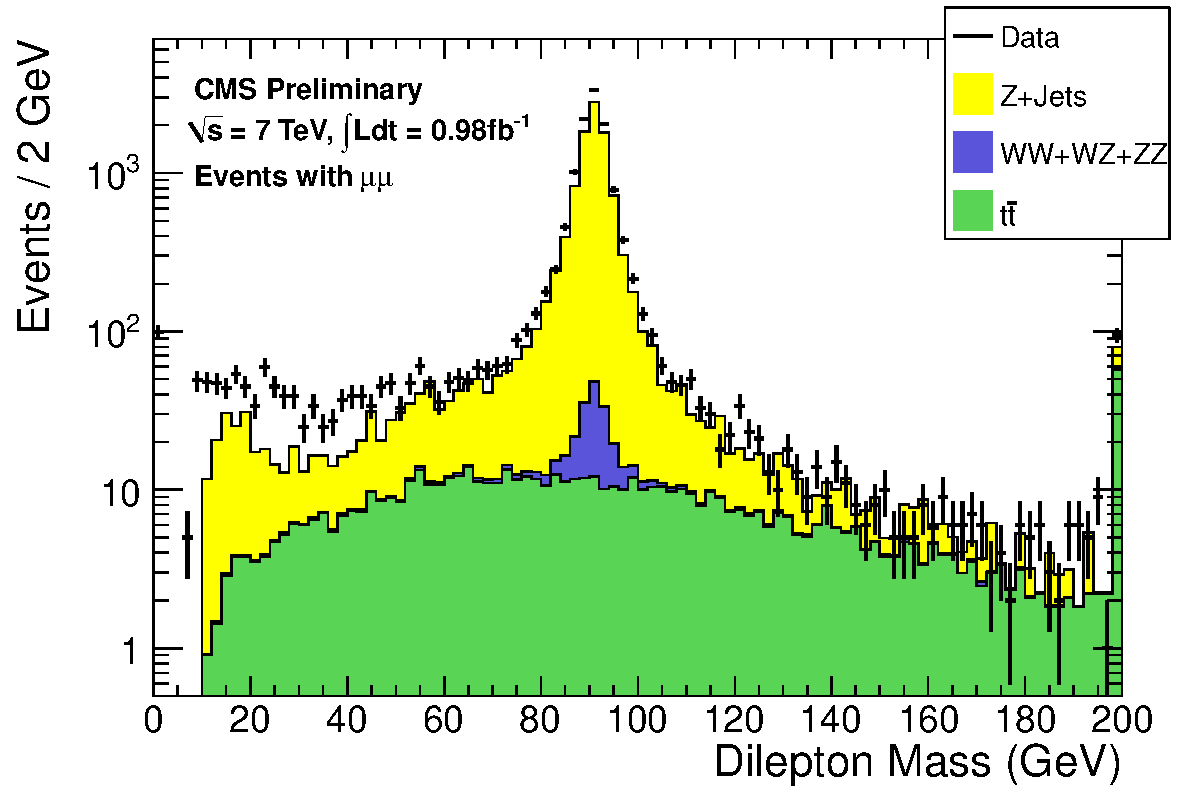
\includegraphics[width=0.48\linewidth]{plots/hdilmass_mm_allj.pdf}
	\caption{
	  \label{fig:dilmass}\protect 
	  Dilepton mass distribution for events passing the pre-selection for \lumi~
	  in the $ee$ (left) and $\mu\mu$ (right) final states. Backgrounds from 
	  single top and $W$+jets are omitted
	  since they are negligible.}
  \end{center}
\end{figure}


The data yields and the MC predictions are given in Table~\ref{preselyieldtable}, after applying
the full preselection including the dilepton mass requirement.
%Dilepton mass and MET distributions for \emu ~events are shown in appendix \ref{app:emu}.
As anticipated, the MC predicts that the preselection is dominated by Z+jets in the same-flavor 
case and by \ttbar\ in the opposite-flavor case. We observe a small deficit %($\sim$9\%) %now ~20%...
in data
with respect to the MC prediction which is dominated by \zjets, but we do not use the \zjets\ MC quantitatively in the search.

%The data yield is in reasonable agreement with the predictions for the $ee$, $\mu\mu$ and $e\mu$ channels.


\begin{table}[htb]
\begin{center}
\caption{\label{preselyieldtable} Data and Monte Carlo yields for the preselection with \njets\ $\ge$ 2 for \lumi. 
}
\begin{tabular}{lccccc}
\hline
              Sample   &                $ee$   &            $\mu\mu$   &              $e\mu$   &         tot  \\
\hline
%Normalizing yield tables to 4.98/fb
%Yields for: hyp_z && !hyp_samesign && pfnjet_res >= 2 && (hyp_p4.M() > 81 && hyp_p4.M() < 101) && pfnbtag_tche100 == 0 && nlep == 2 && pfjets_masslead > 70.000000 && pfjets_masslead < 110.000000
%applying b mistag weight
%applying nvtx weight
\hline
        WJets &    2.3 $\pm$    2.2  &     0.0 $\pm$    0.0  &     0.0 $\pm$    0.0  &     2.3 $\pm$    2.2 \\ 
           WW &    2.1 $\pm$    0.2  &     2.6 $\pm$    0.2  &     4.9 $\pm$    0.3  &     9.7 $\pm$    0.5 \\ 
           WZ &  136.8 $\pm$    1.2  &   137.5 $\pm$    1.2  &     0.7 $\pm$    0.1  &   275.1 $\pm$    1.7 \\ 
           ZZ &  121.8 $\pm$    0.9  &   125.6 $\pm$    0.8  &     0.1 $\pm$    0.0  &   247.5 $\pm$    1.2 \\ 
   Single Top &    1.0 $\pm$    0.2  &     1.1 $\pm$    0.3  &     1.7 $\pm$    0.3  &     3.8 $\pm$    0.5 \\ 
       \ttbar &    9.2 $\pm$    0.4  &     9.1 $\pm$    0.4  &    19.1 $\pm$    0.5  &    37.4 $\pm$    0.7 \\ 
       Z+Jets & 10951.2 $\pm$   80.6  &  11566.7 $\pm$   78.7  &     1.8 $\pm$    0.9  &  22519.6 $\pm$  112.7 \\ 
\hline
     Total MC & 11224.4 $\pm$   80.7  &  11842.7 $\pm$   78.7  &    28.4 $\pm$    1.2  &  23095.5 $\pm$  112.7 \\ 
\hline
         Data &   9734  &   10314  &      28  &   20076 \\ 
\hline
\end{tabular}
\end{center}
\end{table}


\begin{comment}

%nj3

Because we consider a signal region selection of \njets\ $\ge$ 3, we show in 
table \ref{preselyieldtablenj3} 
the yields for the preselection with this \njets\ requirement.


\begin{table}[htb]
\begin{center}
\caption{\label{preselyieldtablenj3} Data and Monte Carlo yields for the preselection with \njets\ $\ge$ 3 for \lumi. 
  %The NLO yields for the SUSY benchmark processes LM4 and LM8 are also shown.
}
\begin{tabular}{lccccc}
\hline
Sample & $ee$ & $\mu\mu$ & $e\mu$ & tot \\ 
\hline

        WJets &    0.0 $\pm$    0.0  &     0.0 $\pm$    0.0  &     1.7 $\pm$    1.7  &     1.7 $\pm$    1.7 \\ 
           WW &    3.7 $\pm$    0.3  &     4.0 $\pm$    0.3  &     7.4 $\pm$    0.4  &    15.2 $\pm$    0.5 \\ 
           WZ &  118.1 $\pm$    1.0  &   117.8 $\pm$    0.9  &     1.4 $\pm$    0.1  &   237.3 $\pm$    1.3 \\ 
           ZZ &   71.0 $\pm$    0.6  &    79.2 $\pm$    0.6  &     0.2 $\pm$    0.0  &   150.5 $\pm$    0.8 \\ 
   Single Top &    8.0 $\pm$    0.6  &     7.0 $\pm$    0.5  &    14.2 $\pm$    0.8  &    29.1 $\pm$    1.1 \\ 
   \ttbar &  237.1 $\pm$    1.7  &   238.3 $\pm$    1.7  &   479.1 $\pm$    2.4  &   954.4 $\pm$    3.4 \\ 
       Z+Jets & 9932.0 $\pm$   65.1  &  10147.2 $\pm$   62.4  &     5.3 $\pm$    1.5  &  20084.4 $\pm$   90.2 \\ 
\hline
     Total MC & 10369.8 $\pm$   65.1  &  10593.5 $\pm$   62.4  &   509.3 $\pm$    3.4  &  21472.6 $\pm$   90.3 \\ 
\hline
         Data &   9760  &   10356  &     506  &   20622 \\ 

\end{tabular}
\end{center}
\end{table}

\end{comment}
